\documentclass{article}
\usepackage{CJKutf8}
\usepackage{enumitem}   
\usepackage{graphicx}
\usepackage{ amssymb }
\usepackage{listings}

\usepackage{listings}
\usepackage{color}

\definecolor{dkgreen}{rgb}{0,0.6,0}
\definecolor{gray}{rgb}{0.5,0.5,0.5}
\definecolor{mauve}{rgb}{0.58,0,0.82}

\lstset{ %
  language=Octave,                % the language of the code
  basicstyle=\footnotesize,           % the size of the fonts that are used for the code
  numbers=left,                   % where to put the line-numbers
  numberstyle=\tiny\color{gray},  % the style that is used for the line-numbers
  stepnumber=2,                   % the step between two line-numbers. If it's 1, each line 
                                  % will be numbered
  numbersep=5pt,                  % how far the line-numbers are from the code
  backgroundcolor=\color{white},      % choose the background color. You must add \usepackage{color}
  showspaces=false,               % show spaces adding particular underscores
  showstringspaces=false,         % underline spaces within strings
  showtabs=false,                 % show tabs within strings adding particular underscores
  frame=single,                   % adds a frame around the code
  rulecolor=\color{black},        % if not set, the frame-color may be changed on line-breaks within not-black text (e.g. commens (green here))
  tabsize=2,                      % sets default tabsize to 2 spaces
  captionpos=b,                   % sets the caption-position to bottom
  breaklines=true,                % sets automatic line breaking
  breakatwhitespace=false,        % sets if automatic breaks should only happen at whitespace
  title=\lstname,                   % show the filename of files included with \lstinputlisting;
                                  % also try caption instead of title
  keywordstyle=\color{blue},          % keyword style
  commentstyle=\color{dkgreen},       % comment style
  stringstyle=\color{mauve},         % string literal style
  escapeinside={\%*}{*)},            % if you want to add LaTeX within your code
  morekeywords={*,...}               % if you want to add more keywords to the set
}

\begin{document}
 
\begin{CJK*}{UTF8}{gbsn}
 

 \begin{enumerate}[label=(\roman*)]
\item \textbf{设计一个神经网络,让其实现加法器的功能,并给出网络结构。网络的输入和输出如
下图示例(RNN,144 + 177 = 321)}
\item \textbf{设计一个神经网络做数字分类任务}

\begin{enumerate}
	\item 网络结构
	\begin{figure}[h]
	  \centering
	      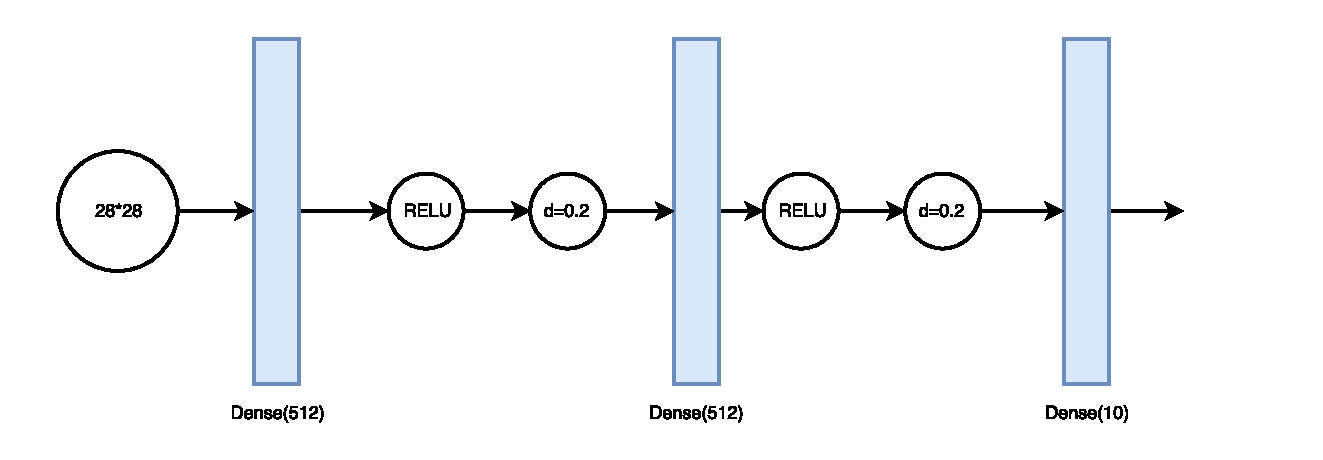
\includegraphics[width=\textwidth]{MNIST.pdf}
	  \caption{MLP结构}
	\end{figure}

	\begin{figure}[h]
	  \centering
	      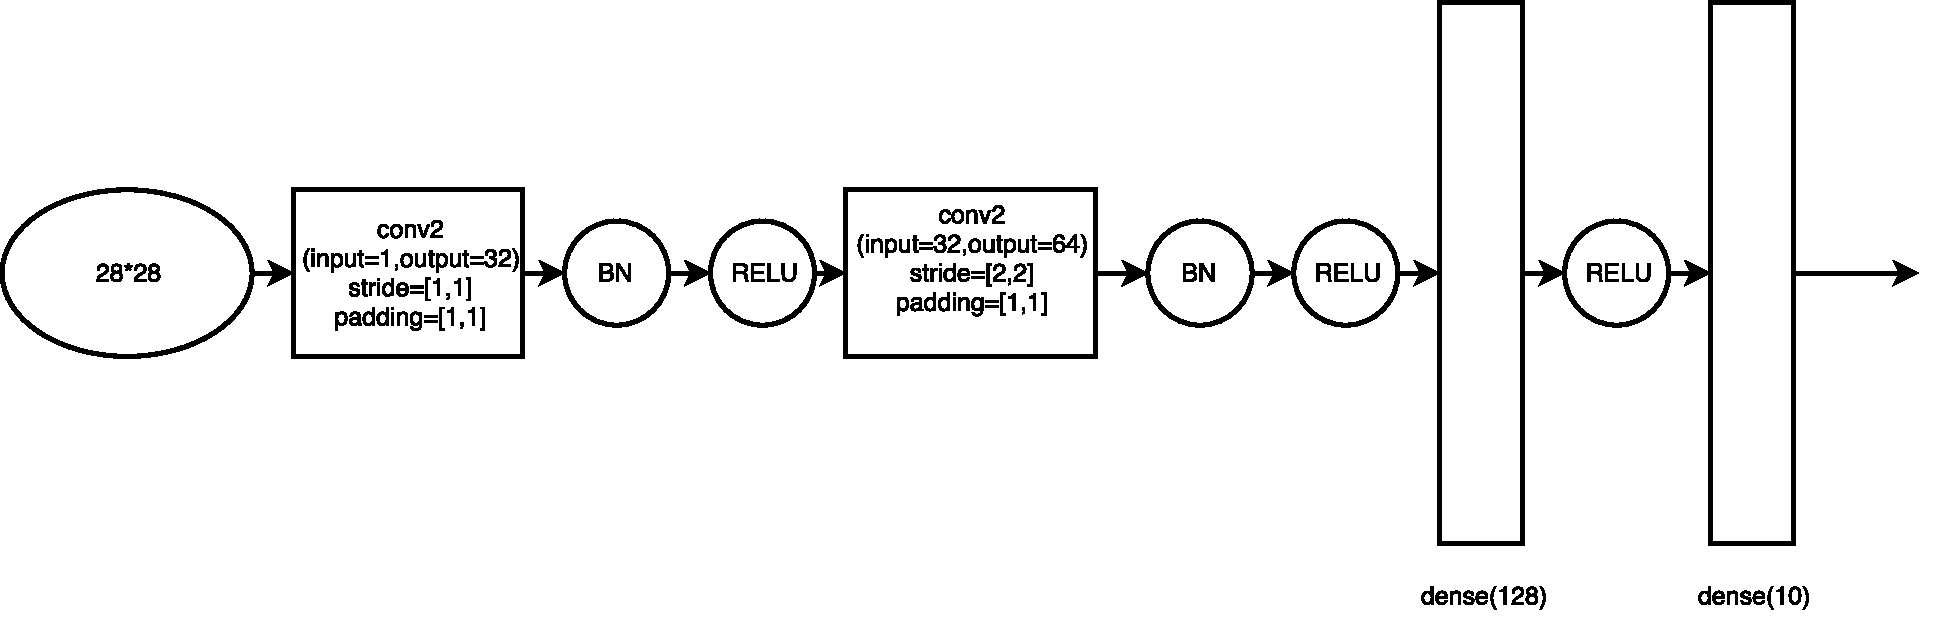
\includegraphics[width=\textwidth]{MNIST2.pdf}
	  \caption{CNN结构}
	\end{figure}

	\begin{table}[h]
	\centering
	\caption{性能比较}
	\label{my-label}
	\begin{tabular}{ccccccc}
	\hline
	 Network & use BN & use Dropout & iteration & time & accuracy &  \\
	 MLP &            &             & 10000($\approx$20eps) &      & 97.67\%  & \\
	 MLP & \checkmark &             & 10000($\approx$20eps)&      & 98.57\%  & \\
	 MLP & \checkmark & \checkmark  & 10000($\approx$20eps)&      & 97.67\%  & \\
	 CNN &          &             & 10000($\approx$20eps)&      & 98.62\%  & \\
	 CNN & \checkmark &             & 10000($\approx$20eps)&      & 97.67\%  & \\
	 CNN &            & \checkmark  & 10000($\approx$20eps)&      & 99.16\%  & \\
	 CNN & \checkmark & \checkmark  & 10000($\approx$20eps)&      & 97.67\%  & \\

	\end{tabular}
	\end{table}
	\item train执行命令:
		\begin{lstlisting}[]
			python Main.py
		\end{lstlisting}
	\item
\end{enumerate}


\item \textbf{自己训练DL中遇到过最难的问题是什么?怎么解决的?}
\item \textbf{开放题:如何看待《DL是个黑盒子》?}
\end{enumerate}

\end{CJK*}
 
\end{document}